% ****** Start of file apssamp.tex ******
%
%   This file is part of the APS files in the REVTeX 4.1 distribution.
%   Version 4.1r of REVTeX, August 2010
%
%   Copyright (c) 2009, 2010 The American Physical Society.
%
%   See the REVTeX 4 README file for restrictions and more information.
%
% TeX'ing this file requires that you have AMS-LaTeX 2.0 installed
% as well as the rest of the prerequisites for REVTeX 4.1
%
% See the REVTeX 4 README file
% It also requires running BibTeX. The commands are as follows:
%
%  1)  latex apssamp.tex
%  2)  bibtex apssamp
%  3)  latex apssamp.tex
%  4)  latex apssamp.tex
%
\documentclass[%
 reprint,
%superscriptaddress,
%groupedaddress,
%unsortedaddress,
%runinaddress,
%frontmatterverbose, 
%preprint,
%showpacs,preprintnumbers,
%nofootinbib,
%nobibnotes,
%bibnotes,
 amsmath,amssymb,
 aps,
%pra,
%prb,
%rmp,
%prstab,
%prstper,
%floatfix,
showkeys
]{revtex4-1}

\usepackage[demo]{graphicx}% Include figure files
\usepackage{dcolumn}% Align table columns on decimal point
\usepackage{bm}% bold math
%\usepackage{hyperref}% add hypertext capabilities
%\usepackage[mathlines]{lineno}% Enable numbering of text and display math
%\linenumbers\relax % Commence numbering lines

%\usepackage[showframe,%Uncomment any one of the following lines to test 
%%scale=0.7, marginratio={1:1, 2:3}, ignoreall,% default settings
%%text={7in,10in},centering,
%%margin=1.5in,
%%total={6.5in,8.75in}, top=1.2in, left=0.9in, includefoot,
%%height=10in,a5paper,hmargin={3cm,0.8in},
%]{geometry}

%Paquetes que yo agregué
\usepackage[utf8]{inputenc}
\usepackage[spanish]{babel}
\usepackage[sort&compress]{natbib}
\usepackage{graphicx}% Include figure files, es demo para saber q la gráfica va ahí. Latex pone un cuadro negro

\begin{document}

\preprint{APS/123-QED}

\title{Relación filogenética de bacterias pertenecientes a la familia Enterobacteriaceae por medio de electroforesis SDS-PAGE en Gel de Policrilamida Vertical}% Force line breaks with \\
\thanks{Laboratorio de Biología Molecular - Artículo 1}%

\author{Angie Ramos}
% \altaffiliation[Also at ]{Physics Department, XYZ University.}%Lines break automatically or can be forced with \\
\author{Daniel Molano}%
 %\email{Second.Author@institution.edu}
\author{Elkin Alvis}
% \altaffiliation[Also at ]{Physics Department, XYZ University.}%Lines break automatically or can be forced with \\
\author{Sof\'ia Ardila}
% \altaffiliation[Also at ]{Physics Department, XYZ University.}%Lines break automatically or can be forced with \\

\affiliation{ Universidad de los Andes\\ 
 Bogotá D.C. - Colombia}%


\date[Fecha: ]{\today}% It is always \today, today,
             %  but any date may be explicitly specified

\begin{abstract}
Aquí va el resumen
\end{abstract}

\pacs{Valid PACS appear here}% PACS, the Physics and Astronomy
                             % Classification Scheme.
\keywords{Cromatografía, Electroforesis en Gel Vertical, Gel de Policrilamida, SDS-PAGE, Tinción, Azul de Coomasie}%Use showkeys class option if keyword
                              %display desired
\maketitle

%\tableofcontents

\section{\label{sec:Intro}Introducción}
	Aquí hay q escribir la introducción de nuestro artículo\citep{Alfonso2010a}. \\

	
	\begin{itemize}
		\item Identificar nítidamente el problema.
		\subitem Resaltar trabajos y contribuciones de otros autores respecto al tema objeto.
		\item Justificación.
		\item Hipótesis. 
		\item Objetivos.
	\end{itemize}
	
	
\section{\label{sec:MyM}Materiales y Métodos}
	Para este estudio se utilizaron proteínas bacterianas de \textit{Escherichia coli}(\textit{E. Coli})K12, \textit{E. Coli}C600, ,  todas pertenecientes a la familia enterobacteriaceae; a continuación se enuncian los pasos seguidos para determinar su relación filogenética.
	Primero se realizó la extracción de proteínas de las células correspondientes, luego se realizó una electroforesis SDS-PAGE en gel de policrilamida vertical y se procedió a teñir con azul de Coomasie. Se analizó el patrón de bandas obtenido utilizando la herramienta computacional \textit{PAUP} obteniendo finalmente los fenogramas correspondientes, con los cuales se pudo determinar la relación filogenética entre las bacterias estudiadas. A continuación se describe en detalle cada uno de los procedimientos enunciados.
	
	\subsection{\label{sec:ExtraMet}Extracción de Proteínas Bacterianas}
		El primer paso para determinar las relaciones filogenéticas de las bacterias en estudio es extraer las proteínas de las células.
		Se comienza dejando las bacterias en crecimiento ON (Over Night) en caldo LB con una agitación de 250$rpm$. Una vez terminado el crecimiento, se procede a medir con una micropipeta 1$ml$ de cada uno de los cultivos y se colocan en \textit{eppendorfs} individuales. Se centrifugan las muestras a 13$Mrpm$ durante 5 minutos; seguidamente, se descarta 800$\mu l$ de la solución en hipoclorito diluido. Los 200$\mu l$ restantes fueron se resuspenden con vórtex. Se añade, a continuación, 100$\mu l$ de \textit{buffer} (contiene SDS), correspondientes a $\frac{1}{2}$ del volumen de cada una de las soluciones con las muestras en los eppendorfs. Luego éstos se pusieron en una plancha de calentamiento durante 5 minutos a 100$^{\circ}C$. Posteriormente se centrifugaron a 13$Mrpm$ por 5 minutos, y finalmente, se extraen de cada una de las muestras el sobrenadante donde se encuentran las proteínas de interés.
		
	%	Es importante mencionar que el \textit{buffer} utilizado contenía detergente SDS (Sodium bla bla) que adiciona la carga negativa a la muestra.También es pertinente resaltar que la presencia del glicerol fue fundamental para evitar la formación de cristales y el congelamiento que podían alterar a muestra, de igual muestra, el azul de bromofenol fue relevante al permitir visualizar el frente de corrido. 
			
	\subsection{\label{sec:ElectroMet}Electroforesis en geles de Policrilamida}		
		Posterior a la extracción de proteínas se procede a realizar la electroforesis en geles de policrilamida vertical. 
		
		Se comienza preparando los geles. El primero a preparar es el gel de separación; se prepara este gel a una concentración del 10\% debido a que las proteínas en cuestión se encuentran en el rango de 16-70$KDa$. El primer paso es mezclar en un beaker 2$ml$ de solución de policrilamida, 1.25$ml$ de una solución con pH 8.8 y 1.75$ml$ de $H_2O$. A continuación se adicionan simultáneamente 50$\mu l$ de persulfato de amonio al 10\% y 8$\mu l$ de TEMED. Inmediatamente se vierte dentro de la cámara del montaje y se deja polimerizar unos 45 minutos. Para el gel de agrupamiento, se comienza mezclando en un beaker 325$\mu l$ de policrilamida, 625$\mu l$ de una solución con pH 6.8 y 1525$\mu l$ de $H_2O$. Luego se adiciona simultáneamente 25$\mu l$ de persulfato de amonio al 10\% y 5$\mu l$ de TEMED, se agita bien y se vierte en la cavidad del montaje, se ponen los peines para crear los pozos y se deja polimerizar por 15 minutos. Transcurrido este tiempo se pueden retirar los peines y proceder con el montaje de la cámara de electroforesis. El montaje debe verse similar al mostrado en la figura \ref{Imagen: SDS-PAGE}.
		
		\begin{figure}[h]
		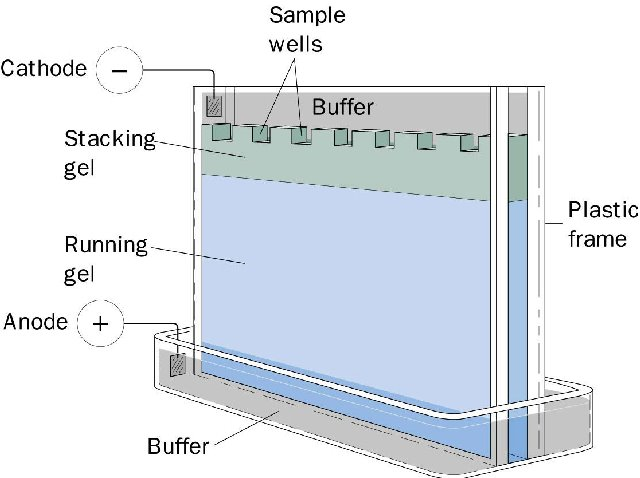
\includegraphics[width=0.4\textwidth]{SDS-PAGE.jpg}
		\caption{SDS-PAGE}
		\label{Imagen: SDS-PAGE}
		\end{figure} 

		Para realizar el montaje de la cámara electroforética, se asegura el o los pares de geles en el interior de esta. Se llena la cámara interna con \textit{buffer} de electroforesis 1X hasta que cubra los pozos y vierta el resto del \textit{buffer} en la cámara externa. Se continúa sembrando 8$\mu l$ de cada una de las muestras. Terminado el sembrado, se cierra apropiadamente la cámara y se programa el corrido de electroforesis a 150$V$ y 90 minutos. Una vez terminado el corrido se procede a fijarlo. Para esto se prepara una solución de fijado, que se compone de 50\% de etanol, 10\% de ácido acético y 40\% de $dH_2O$. Esta solución se vierte en las cubetas del kit y a continuación se desmonta el gel de la cámara. Primero se apaga y desconecta la fuente de poder, se retira el montaje de los vidrios y se separa con cuidado el gel de estos. Se separa y se descarta el gel de agrupamiento y se hace un pequeño corte en alguna esquina para identificar la ubicación del primer carril del gel. A paso seguido se deposita el gel en la cubeta con la solución de fijado y se guarda la el gel a 4$^{\circ}C$ por 8 días.

		Nota: Cabe resaltar que en el gel se siembran proteínas de 2 bacterias más: bla1 y bla2. Estas fueron suministradas por el docente al momento de la siembra.
		
	\subsection{\label{sec:TinMet}Tinción con Azul de Coomasie}	
		Una vez el gel esté fijado, se tiñe con Azul de Coomasie para ver el patrón de bandeo.
		
		Se prepara la solución de tinción mezclando 50\% de metanol, 10\% de ácido acético, 40\% de $dH_2O$ y Coomasie al 0.05\%. Se Retira la solución de fijación de la cubeta, cuidando que el gel no quede con pliegues, se agrega la solución de tinción y se deja en agitación continua a aproximadamente 60$rpm$ y 37$^{\circ}C$ durante 45 minutos. Transcurrido el tiempo, se descarta la solución de tinción y se hace un lavado $dH_2O$. Seguido de esto, se agrega la solución de destinción previamente preparada así: 50\% de metanol, 10\% de ácido acético y 40\% de $dH_2O$. La cubeta con el gel en la solución de destinción, se deja en agitación constante a 50$rpm$ y 37$^{circ}C$ hasta que se obtiene la intensidad de las bandas deseada.
		
		Obtenido el bandeo deseado, se retira el gel de la solución de destinción y se pone a secar en papel celofán en frío toda una noche.
		
	\subsection{\label{sec:Fen}Construcción del fenograma}	
		Una vez seco el gel, se procede al reconocimiento y conteo de bandas para su análisis utilizando \textit{PAUP}.
		
	
\section{\label{sec:Resul}Resultados}

	\begin{figure}[h]
	\includegraphics[width=0.4\textwidth]{geli.jpg}
	\caption{Gel I}
	\label{Imagen: gelI}
	\end{figure} 
	
	\begin{figure}[h]
	\includegraphics[width=0.4\textwidth]{gelii.jpg}
	\caption{Gel II}
	\label{Imagen:gelII}
	\end{figure} 
	
	\subsection{La matriz}
	
	\begin{table}[h]
		\centering
		\large
		\caption{Matriz.}
		\label{tabla:autores}
		
		\begin{tabular}{|l||l|l|l|l|l|l|l|l|l|} \hline
		\textbf{Banda} & \textbf{1} & \textbf{2} & \textbf{3} & \textbf{4} & \textbf{5} & \textbf{6} & \textbf{7} & \textbf{8} & \textbf{9}\\ \hline \hline
		\textbf{Organismo 1} & 1 & 1 & 1 & 1 & 1 & 1 & 1 & 0 & 1\\ \hline
		\textbf{Organismo 2} & 1 & 1 & 1 & 1 & 1 & 1 & 1 & 0 & 1\\ \hline
		\textbf{Organismo 3} & 1 & 1 & 1 & 1 & 1 & 1 & 1 & 0 & 1\\ \hline
		\textbf{Organismo 4} & 1 & 1 & 1 & 1 & 1 & 1 & 1 & 0 & 1\\ \hline
		\textbf{Organismo 5} & 0 & 0 & 0 & 0 & 0 & 0 & 1 & 1 & 1\\ \hline
		\textbf{Organismo 6} & 1 & 1 & 1 & 1 & 1 & 1 & 1 & 1 & 1\\ \hline
		\end{tabular}
	\end{table}	

	\begin{figure}[h]
	\includegraphics[width=0.4\textwidth]{arbolNj.jpg}
	\caption{Árbol Nj.}
	\label{Grafica:Nj}	
	\end{figure}

	\begin{figure}[h]
	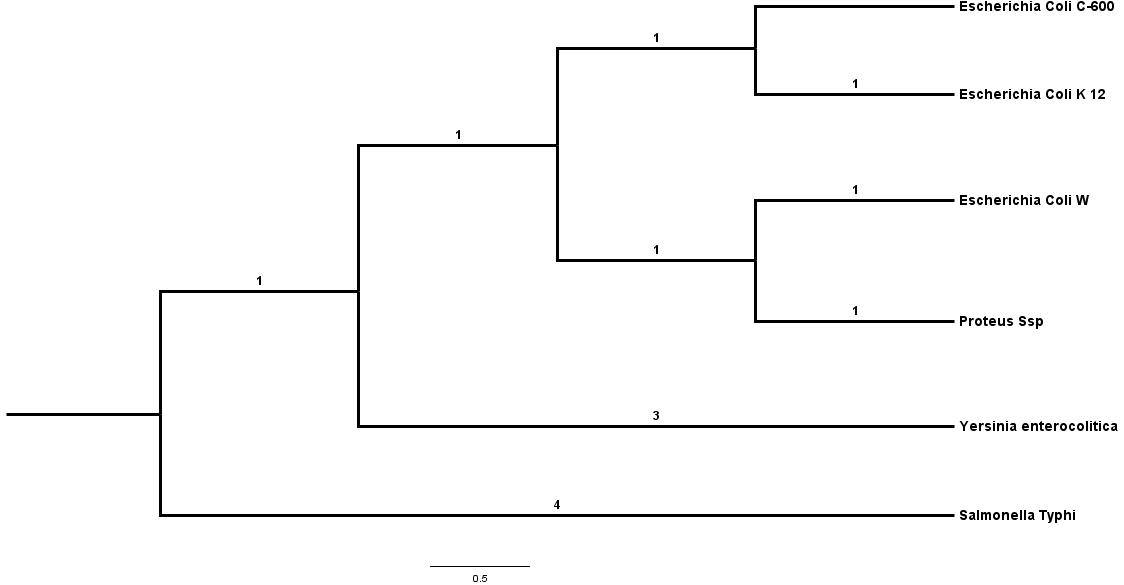
\includegraphics[width=0.4\textwidth]{arbolUPGMA.jpg}
	\caption{Árbol UPGMA}
	\label{Grafica: UPGMA}
	\end{figure}	

\section{\label{sec:Dis}Discusión de Resultados}


\bibliographystyle{apalike}
\bibliography{proteinasBib}
\end{document}
%
% ****** End of file apssamp.tex ******
